\documentclass[18pt, aspectratio=169]{beamer}
\usepackage[utf8]{inputenc}
% \usepackage{templates/mytemplate}
\usepackage{templates/beamerthemekit}
\usepackage{graphicx}
\usepackage{microtype}
\usepackage{xcolor}
\usepackage{hyperref}
\usepackage{multicol}
\usepackage{siunitx}
\usepackage{physics}
\usepackage{appendixnumberbeamer}
\usepackage{booktabs}
\usepackage{longtable}

% for bold rows in tabular
\usepackage{array}
\usepackage{siunitx}
\newcolumntype{X}{%
  >{\rowstyle{\relax}}c%
}
\newcolumntype{Y}{%
  >{\currentrowstyle}S[detect-weight, table-format=6.2]%
}
\newcommand{\rowstyle}[1]{%
  \protected\gdef\currentrowstyle{#1}%
}
\sisetup{detect-weight=true, detect-family=true}

\title{\\Einsichten in die Spurfindung an der Belle~II-Driftkammer mithilfe von kosmischen Strahlen}
\subtitle{DPG Frühjahrstagung 2018}
\author[Michael Eliachevitch]{Florian Bernlochner, Nils Braun, \underline{Michael Eliachevitch}, Thomas Hauth, Martin Heck}
\date[2018-03-19]{19. März 2018}
\titleimage{belle2_aerial_cosmics}
% \titleimage{tracks_wide}
% \titlelogo{belle2-logo}
\titlelogo{belle2-logo}
\institute[Institut für Experimentelle Teilchenphysik (ETP)]{Institut für Experimentelle Teilchenphysik (ETP)}
\newcommand{\kitemph}[1]{\textcolor{kit-green100}{\bf{#1}}}

\begin{document}


\selectlanguage{ngerman}
\begin{frame}
  \titlepage
\end{frame}
\selectlanguage{english}
% \begin{frame}
%   \frametitle{Short Introduction to Belle II}
%   \begin{itemize}
%   \item detector at the SuperKEKB accelerator in Tsukuba, Japan
%   \item $B$-factory:\\
%     e$^+$e$^- \xrightarrow{\sqrt{s} = 10.58\rm\,GeV} \Upsilon(4S) \rightarrow  B\bar{B} \rightarrow \dots$
%   \item wide range of physics goals:
%     \begin{itemize}
%     \item search for \kitemph{new physics} in rare decays
%     \item precision measurements of CP violating phases
%     \item \dots
%     \end{itemize}
%   \end{itemize}
% \end{frame}

\begin{frame}
  \frametitle{The Belle II detector}
  \begin{center}
    \includegraphics<1>[width=0.7\textwidth]{figures/belle2_detector_mylabels.pdf}
    \includegraphics<2->[width=0.7\textwidth]{figures/belle2_detector_mylabels_cdchighlight.pdf}
    \uncover<2->{\includegraphics[width=0.3\textwidth]{figures/cdc_installation.png}}
  \end{center}
\end{frame}

\begin{frame}
  \frametitle{Tracking at Belle II}
  \begin{columns}
    \begin{column}{0.5\textwidth}

      \begin{itemize}
      \item average of 11 tracks in $\Upsilon(4S)$ decays
      \item goal: \kitemph{find all} tracks in event
        % \item \kitemph{Validation} of tracking perfomance required:
        %   \begin{itemize}
        %   \item so far: based on Monte Carlo matching in simulation
        %   \item Can we test it on \kitemph{data}?
        %   \end{itemize}
      \end{itemize}
      \begin{block}{CDC track finding}
        \begin{enumerate}
        \item Global legendre algorithm\\(extended hough-algorithm)
        \item Local cellular automaton\\
        \end{enumerate}
      \end{block}
      \begin{itemize}
      \item Tracking \kitemph{validation}:\\
        based on \kitemph{Monte Carlo-matching}
      \end{itemize}
    \end{column}
    \begin{column}{0.5\textwidth}
      \centering \scriptsize
      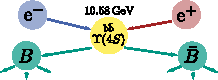
\includegraphics[width=0.65\textwidth]{figures/eplus_eminus_to_b_bar_diagram.pdf}\\
      \includegraphics[width=0.75\textwidth]{figures/b2display_screenshots/y4s_nobackground_edited.png}
    \end{column}
  \end{columns}
\end{frame}

\begin{frame}
  \frametitle{First data: cosmic rays}
  \begin{columns}
    \begin{column}{0.6\textwidth}
      \begin{itemize}
      \item July -- August 2017: \kitemph{first data} of cosmic rays
      \item vertex detectors not installed yet\\
        $\rightarrow$ empty volume in CDC
      \item typical event:\\\kitemph{single track, no beam background}
      \end{itemize}
      \begin{block}{Motivation of my studies:}
        study tracking performance on cosmic data with real hardware
      \end{block}
    \end{column}
    \begin{column}{0.4\textwidth}
      \centering
      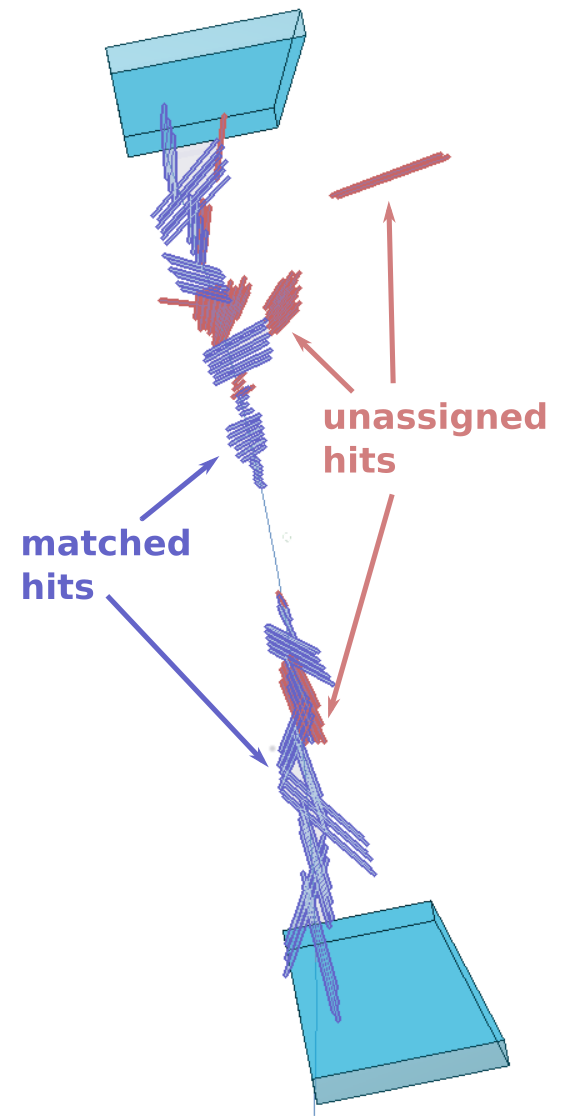
\includegraphics[width=0.65\textwidth]{figures/b2display_screenshots/gcr_mc_2017-08_run3940_evt2754_twotrackevent_3d_annotated.png}
    \end{column}
  \end{columns}


\end{frame}


\begin{frame}
  \frametitle{Study on hit efficiency}
  \begin{columns}
    \begin{column}{0.5\textwidth}
      \begin{itemize}
      \item \textbf{tracking hit efficiency:}\\
        probability that hit is picked up by track finding
      \item \textbf{what we can study on data:}\\
        fraction of hits that belong to a track compared to total hits

        \begin{equation*}
          \frac{N_\mathrm{matched\ hits}}{N_\mathrm{total\ hits}} = \mathrm{hit\ efficiency} \times \frac{N_\mathrm{hits\ from\ tracks}}{N_\mathrm{total\ hits}}
        \end{equation*}
      \item without background, the equality holds
      \end{itemize}

    \end{column}
    \begin{column}{0.5\textwidth}
      \centering
      fraction of hits matched by tracks\\
      \kitemph{on simulated events}\\
      \includegraphics[width=0.9\textwidth]{figures/hit_efficiency_by_wire/gcr1_2017-08/hit_ratio_matched_by_recotrack_MC.png}
    \end{column}
  \end{columns}

\end{frame}

\begin{frame}
  \frametitle{Wire hit efficiency on measured data}
  \begin{columns}
    \begin{column}{0.5\textwidth}
      \centering
      \kitemph{on measured data from August 2017}\\
      \includegraphics[width=0.9\textwidth]{figures/hit_efficiency_by_wire/gcr1_2017-08/hit_ratio_matched_by_recotrack.png}
    \end{column}
    \begin{column}{0.5\textwidth}
      \uncover<2-2>{
        \centering distribution of hits\\
        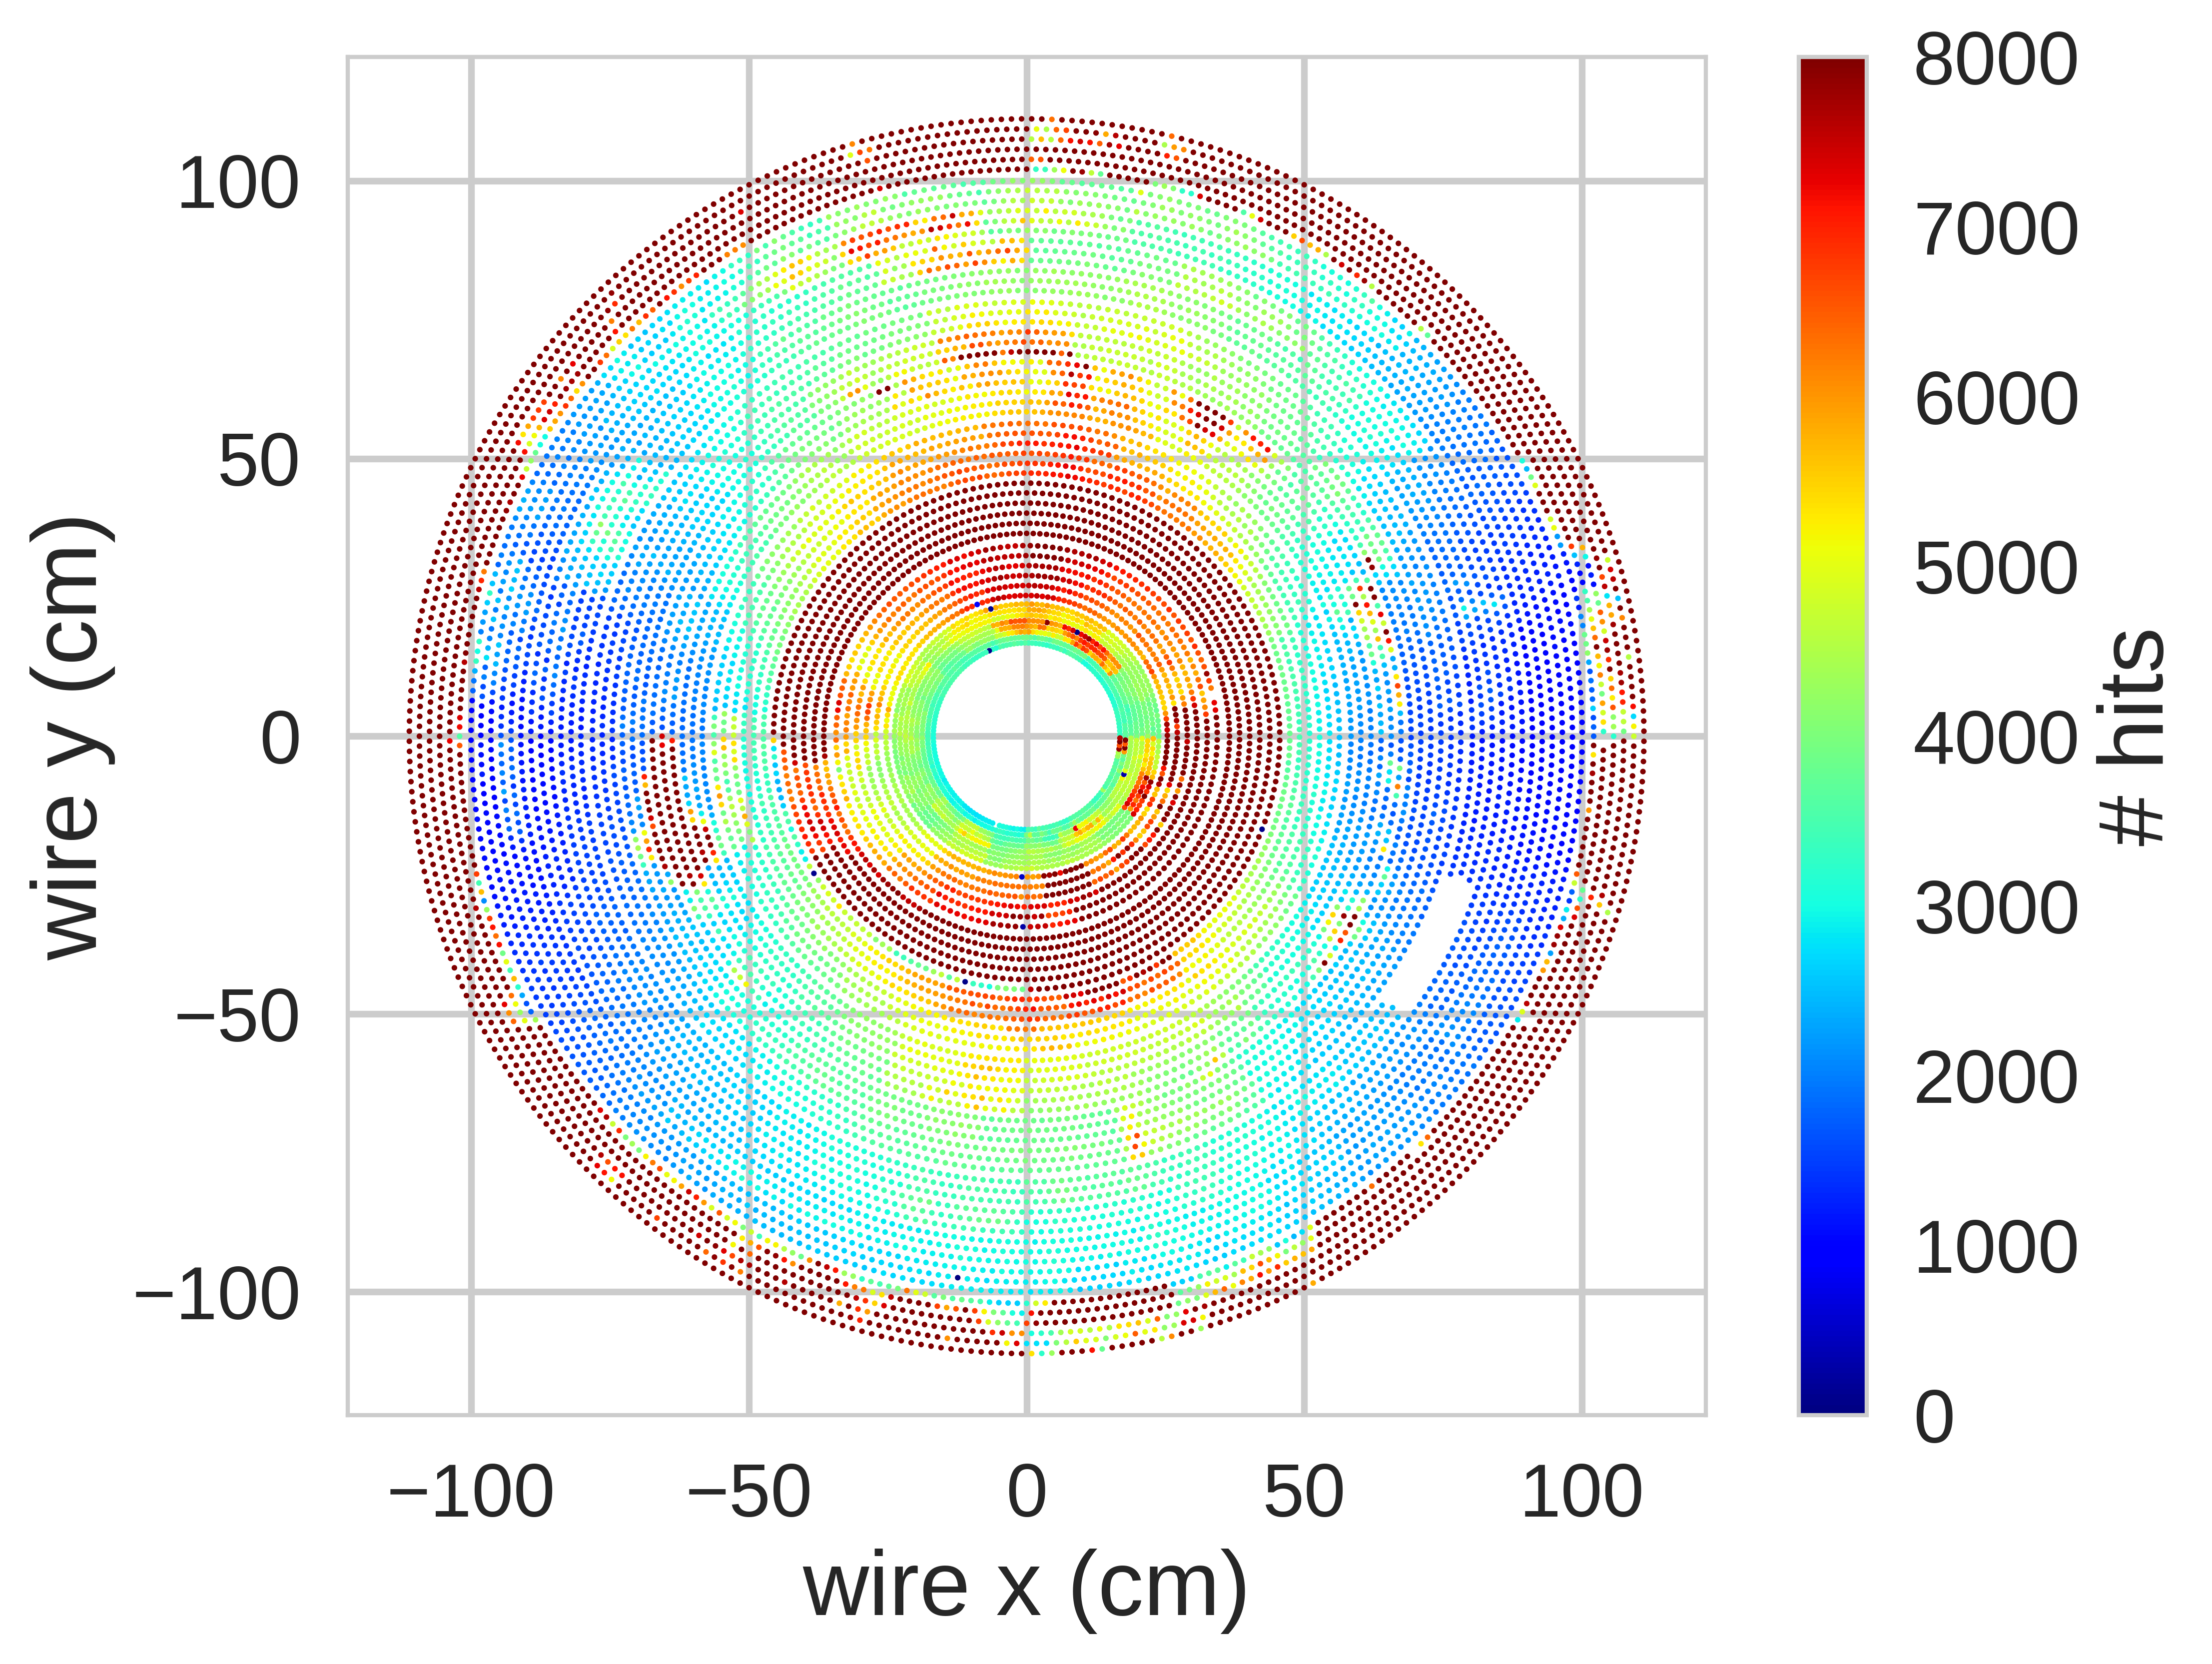
\includegraphics[width=0.9\textwidth]{figures/hit_efficiency_by_wire/gcr1_2017-08/total_hits_per_wire.png}
      }
    \end{column}
  \end{columns}
  \begin{itemize}
  \item noisy regions due to high-voltage issues\\
    $\rightarrow$ has been mostly fixed
  \end{itemize}
\end{frame}

\begin{frame}
  \frametitle{Finding efficiency estimation with cosmic rays}
  \begin{columns}
    \begin{column}{0.5\textwidth}
      \begin{itemize}
      \item CDC has ``hole'' around interaction point
      \item cosmic rays through centre reconstructed as two seperate tracks
      \item \kitemph{select events} with \textcolor{kit-blue100}{two findable tracks}
      \item count  \textcolor{kit-red100}{finding failures}:\\events where only one track is found
      \end{itemize}
    \end{column}
    \begin{column}{0.3\textwidth}
      \centering
      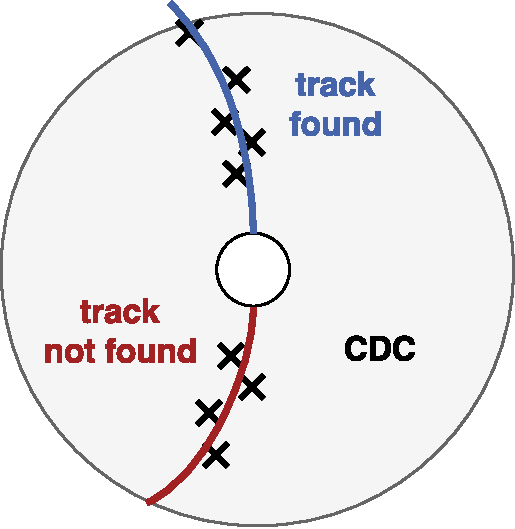
\includegraphics[width=1.0\textwidth]{figures/cdc_finding_fail_diagram.pdf}
    \end{column}
    \begin{column}{0.2\textwidth}
      \centering
      \includegraphics[width=1.0\textwidth]{figures/b2display_screenshots/gcr_data_2017-08_run3940_2326_finding-fail-musterevent_3d.png}
    \end{column}
  \end{columns}

  \begin{equation*}
    \label{eq:cosmic_eff}
    \text{finding efficiency} \approx \frac{N_\mathrm{2\ tracks\ found}}{\textcolor{kit-blue100}{N_\mathrm{2\ tracks\ expected}}}
    = 1 - \frac{\textcolor{kit-red100}{N_\mathrm{1\ track\ found}}}{\textcolor{kit-blue100}{N_\mathrm{2\ tracks\ expected}}}
  \end{equation*}             %
  % where $\textcolor{kit-red100}{N_\mathrm{1\ track\ found}}, N_\mathrm{2\ tracks\ found}, \in \textcolor{kit-blue100}{N_\mathrm{2\ tracks\ expected}}$.\\

\end{frame}

\begin{frame}
  \frametitle{Event selection for finding efficiency estimation}
  \begin{columns}
    \begin{column}{0.5\textwidth}
      \begin{itemize}
      \item \textcolor{kit-blue100}{pre-tracking selection} of events with two
        findable tracks:
        \begin{enumerate}
        \item $85 <$ number of \kitemph{CDC hits} $< 125$
        \item sum of \kitemph{y-positions} of wire hits $< \SI{400}{\cm}$
        \end{enumerate}
      \item only 0.2\% of events with one track (MC truth) in this selection
      \item[$\Rightarrow$] on this selection, count events with only one found track

      \end{itemize}

    \end{column}
    \begin{column}{0.5\textwidth}
      \begin{center}
        \includegraphics<1>[width=0.9\textwidth]{figures/mcsplit_analysis/sum_y_vs_hits_merged_gcraugust_20cm_split.pdf}
        \includegraphics<2>[width=0.9\textwidth]{figures/mcsplit_analysis/sum_y_vs_hits_merged_gcraugust_20cm_split_annotated.pdf}
      \end{center}
      % \begin{itemize}
      % \item ``purity'': 99.8\%% of 358\,k one track events are not in this cut\\
      % \item ``efficiency'': 43.8\%% of 1.288\,M two track events are in this cut
      % \end{itemize}
    \end{column}
  \end{columns}
\end{frame}

\begin{frame}
  \frametitle{Results}
  % \begin{block}{Integrated over all parameter regions}
  %   \begin{tabular}{X|YY}
  %     \toprule
  %     & {measured data} & {simulated data}\\
  %     \midrule
  %     \# one track found & 1281 & 1636 \\
  %     \# two tracks found &  38851 & 599579 \\
  %     \rowstyle{\bfseries} \textbf{``Efficiency'' in \%} & 96.8 & 99.7 \\
  %     \bottomrule
  %   \end{tabular}
  % \end{block}
  \begin{itemize}
  \item ``efficiency'' profiles:\\count finding fails in bins of track parameters
  \end{itemize}
  \begin{columns}
    \begin{column}{0.5\textwidth}
      \centering
      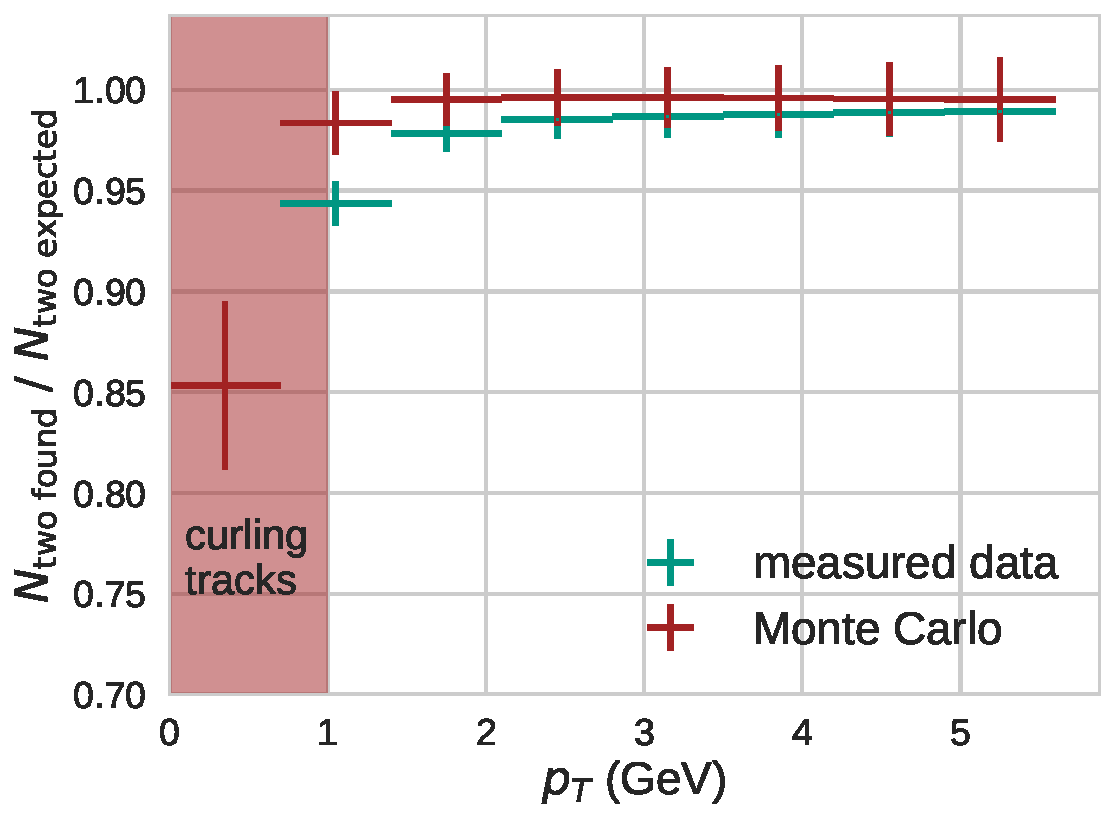
\includegraphics[width=0.8\textwidth]{figures/efficiency_study/cosmicbased_findeff_over_pt_annotated.pdf}
    \end{column}
    \begin{column}{0.5\textwidth}
      \centering
      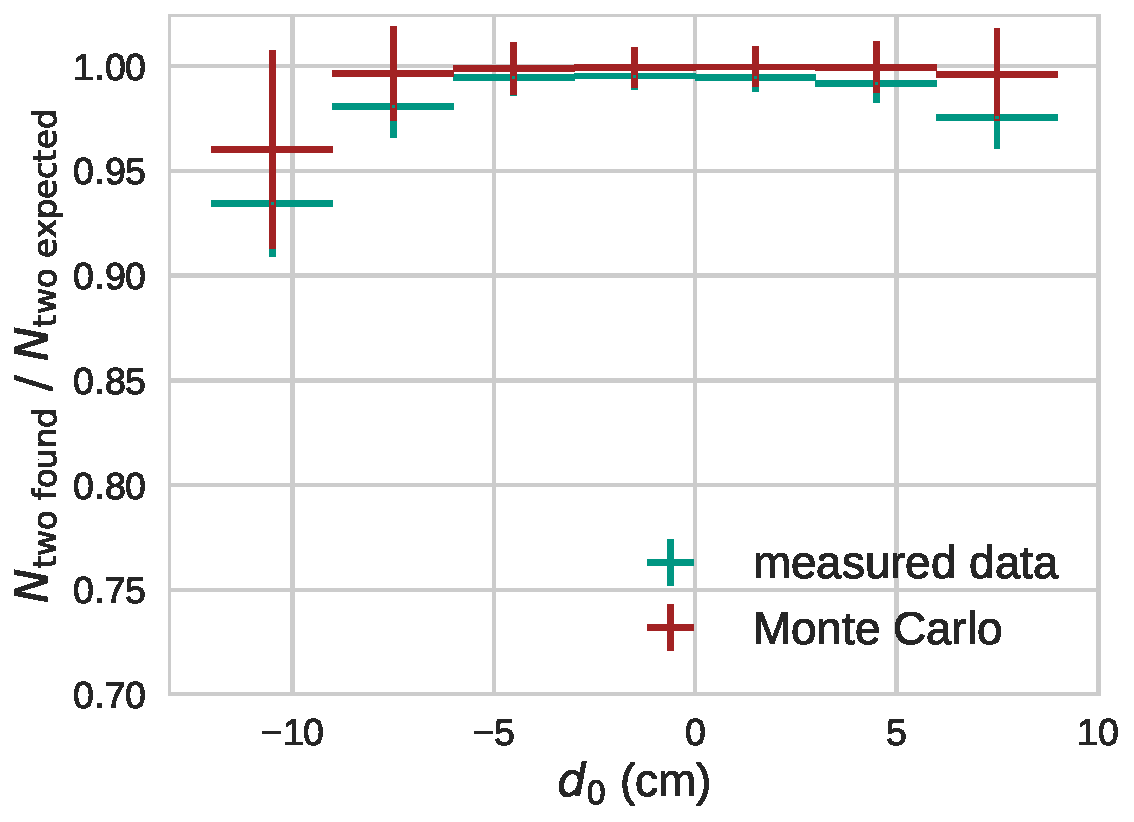
\includegraphics[width=0.8\textwidth]{figures/efficiency_study/cosmicbased_findeff_over_d0.pdf}
    \end{column}
  \end{columns}
  \begin{itemize}
  \item integrated over all parameters in cosmic ray data:
    \begin{itemize}
    \item measured data: 97\%
    \item simulation: 99\%
    \end{itemize}
  \end{itemize}
\end{frame}



\begin{frame}
  \frametitle{Summary and outlook}
  \begin{itemize}
  \item good: high finding efficiency for small impact parameters\\(for which tracking is optimized)
  \item low $p_T$-region: curling tracks, not able to reach CDC centre\\
    $\rightarrow$ method does not work well
  \item better on simulated than on measured data: missing noise in simulation
  \end{itemize}

  \begin{block}{Take home}
    \kitemph{Confirmation, that CDC tracking works on real data and hardware}
    \begin{itemize}
    \item Belle II CDC works
    \item tracking finding algorithms yield expected high efficiency
    \end{itemize}
  \end{block}
  \begin{itemize}
  \item \textbf{Outlook:}
    \begin{itemize}
    \item currently ongoing: cosmic data taking with parts of Vertex
      Detectors
    \item looking forward to first collisions
    \end{itemize}
  \end{itemize}
\end{frame}



\appendix
\backupbegin
\begin{frame}
  % \frametitle{Backup-Folien}
  \centering \huge
  Backup
\end{frame}

% \begin{frame}
%   \frametitle{Summary of all cuts for finding efficiency estimation}
%   \begin{block}{All cuts summarized}
%     \begin{itemize}
%     \item select events where
%       \begin{itemize}
%       \item $85 < \text{number of CDC hits} < 125$
%       \item $\abs{\sum{y}} < \SI{400}{\cm}$
%       \end{itemize}
%     \item require $\abs{\Delta p_T} < \SI{2}{\GeV}$ for two track events
%     \item  cut $d_0$ and $z_0$ impact parameters: $\abs{z_0}_\mathrm{max} < \SI{40}{cm}$ and $\abs{d_0}_\mathrm{max} < \SI{20}{cm}$
%     \end{itemize}
%   \end{block}
% \end{frame}



% \begin{frame}
%   \frametitle{Cosmic track parameter distributions for GCR August 2017 with MC from data production group}
%   \begin{center}
%     \includegraphics[width=0.3\textwidth]{figures/distributions/gcr_august_2017_pt_distribution_normed=True.pdf}
%     \includegraphics[width=0.3\textwidth]{figures/distributions/gcr_august_2017_z0_distribution_normed=True.pdf}
%     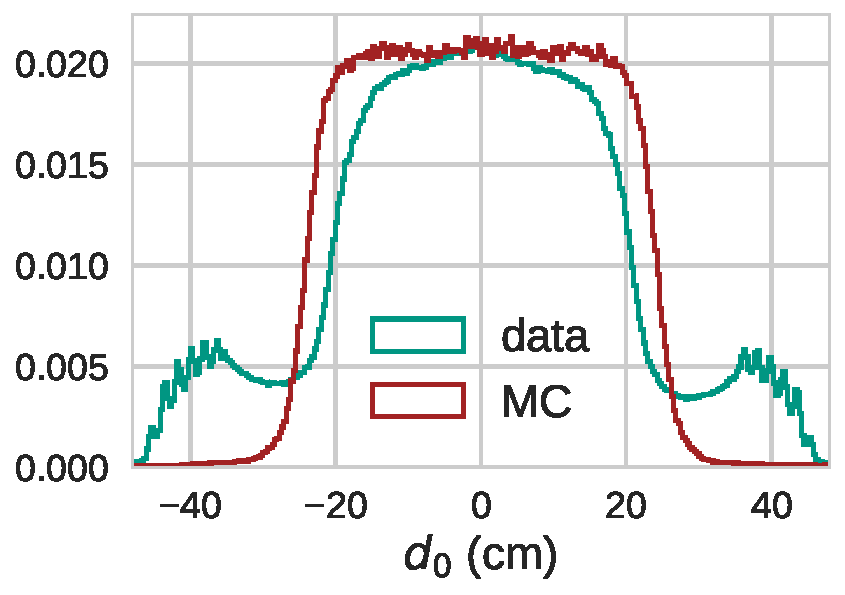
\includegraphics[width=0.3\textwidth]{figures/distributions/gcr_august_2017_d0_distribution_normed=True.pdf}\\
%     \includegraphics[width=0.3\textwidth]{figures/distributions/gcr_august_2017_phi0_distribution_normed=True.pdf}
%     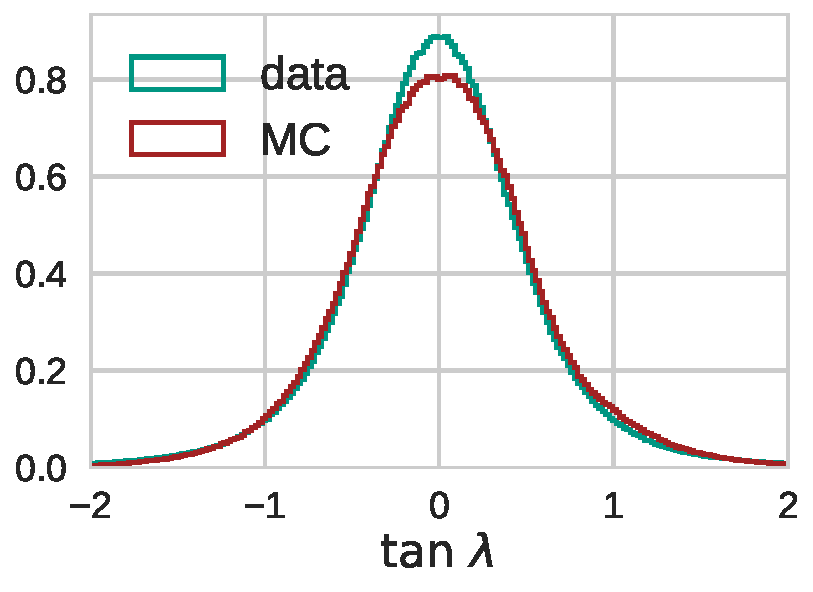
\includegraphics[width=0.3\textwidth]{figures/distributions/gcr_august_2017_tan_lambda_distribution_normed=True.pdf}
%   \end{center}
% \end{frame}

\begin{frame}
  \frametitle{Finding ``efficiency'' profiles in further helix parameters}
  \begin{columns}
    \begin{column}{0.33\textwidth}
      \centering
      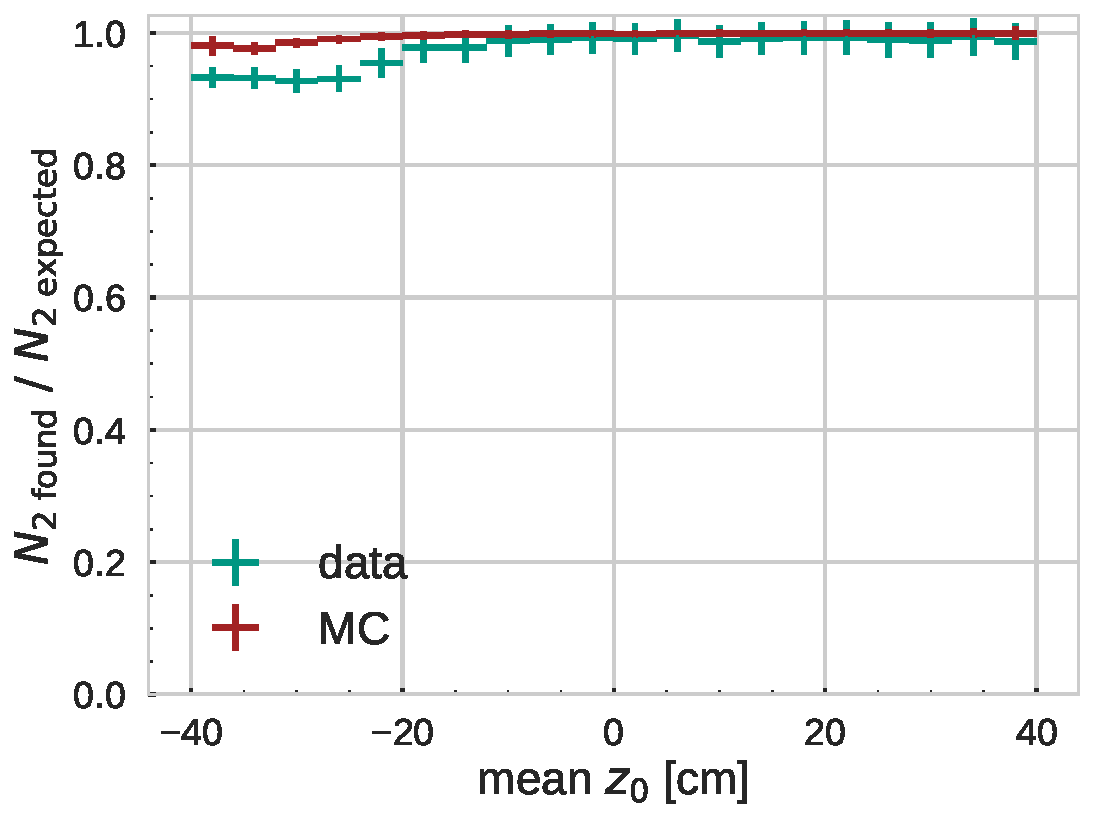
\includegraphics[width=0.9\textwidth]{figures/efficiency_study/cosmicbased_findeff_over_z0.pdf}\\
    \end{column}
    \begin{column}{0.33\textwidth}
      \centering
      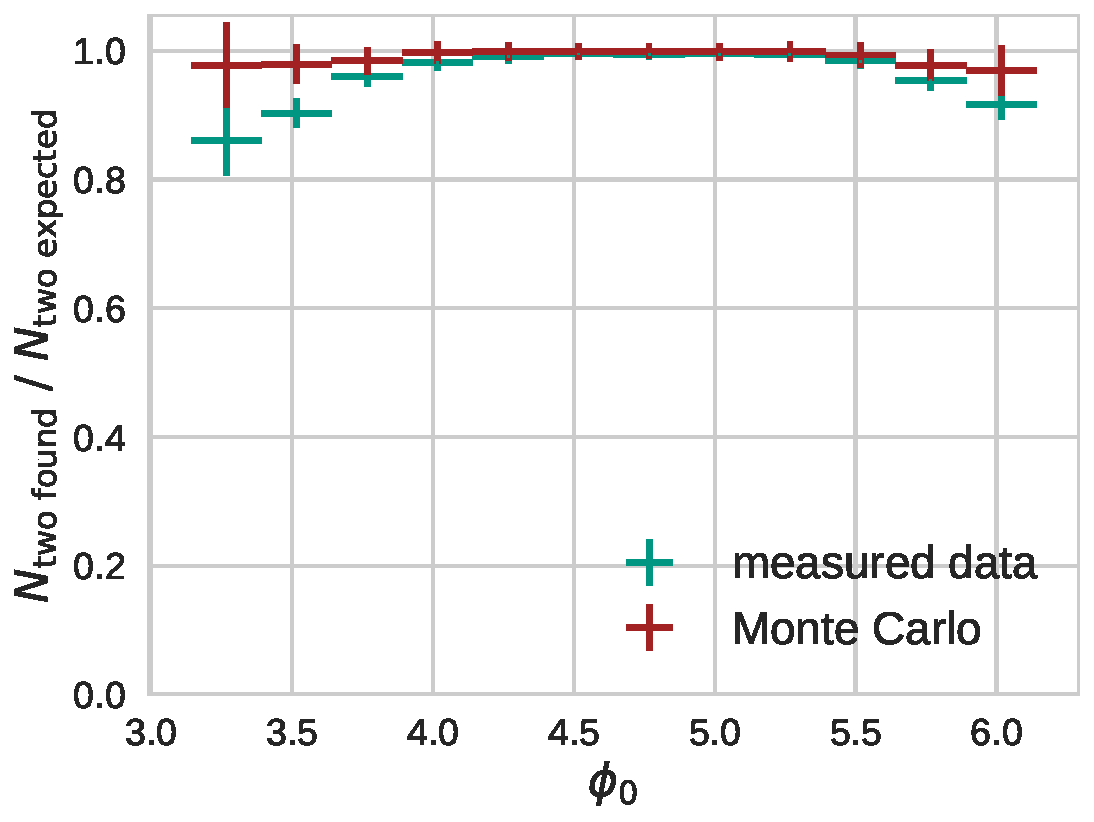
\includegraphics[width=0.9\textwidth]{figures/efficiency_study/cosmicbased_findeff_over_phi0.pdf}\\
    \end{column}
    \begin{column}{0.33\textwidth}
      \centering
      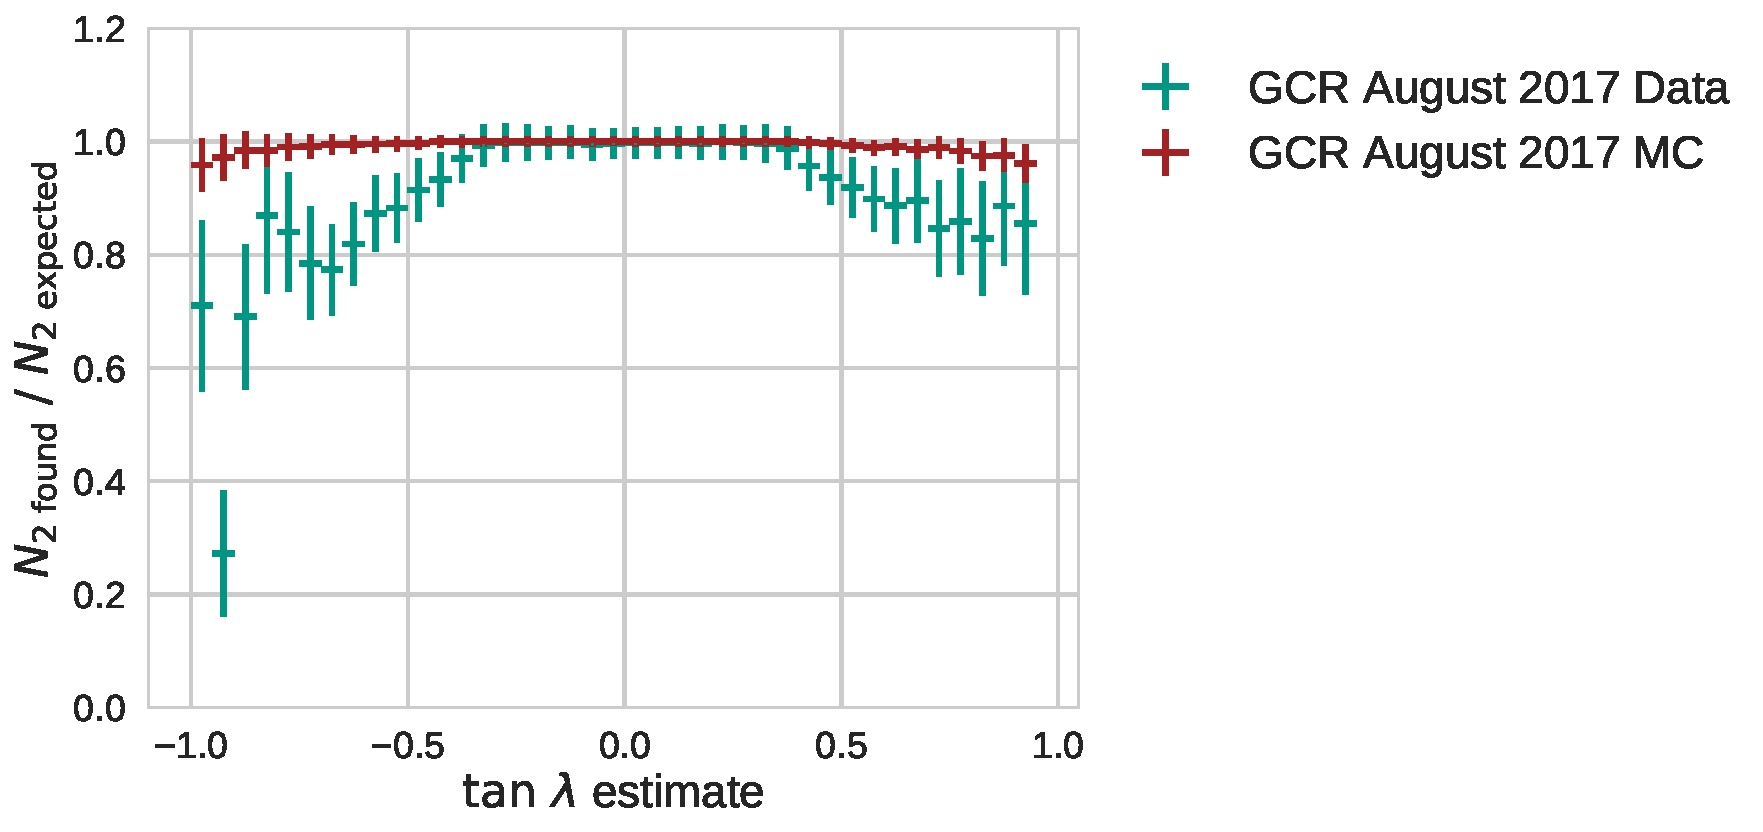
\includegraphics[width=0.9\textwidth]{figures/efficiency_study/cosmicbased_findeff_over_tan_lambda.pdf}
    \end{column}
  \end{columns}
\end{frame}

\begin{frame}
  \frametitle{Wire hit efficiency on  new cosmics data from February 2018}
  \begin{columns}
    \begin{column}{0.5\textwidth}
      \centering
      fraction of hits matched by tracks
      \includegraphics[width=0.9\textwidth]{figures/hit_efficiency_by_wire/gcr2/r00304/hit_ratio_matched_by_recotrack.png}
    \end{column}
    ;\begin{column}{0.5\textwidth}
      \centering distribution of all hits\\
      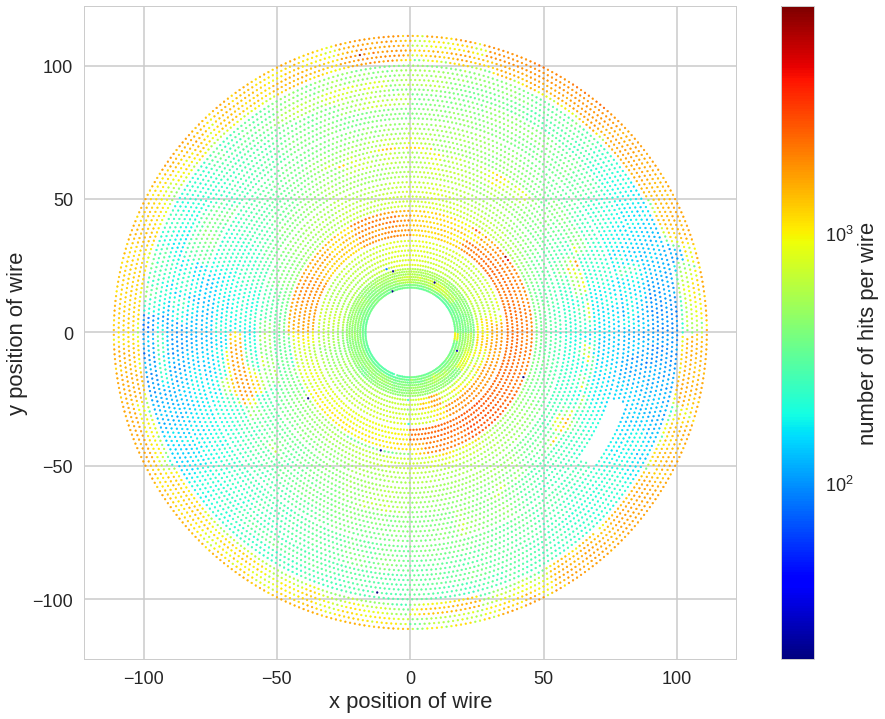
\includegraphics[width=0.9\textwidth]{figures/hit_efficiency_by_wire/gcr2/r00304/total_hits_per_wire.png}
    \end{column}
  \end{columns}
\end{frame}

\begin{frame}
  \frametitle{Cosmic track parameter distributions for GCR August 2017 data and my own MC}
  \begin{center}
    \includegraphics[width=0.3\textwidth]{figures/distributions/gcr_august_2017_pt_distribution_normed=True.pdf}
    \includegraphics[width=0.3\textwidth]{figures/distributions/gcr_august_2017_z0_distribution_normed=True.pdf}
    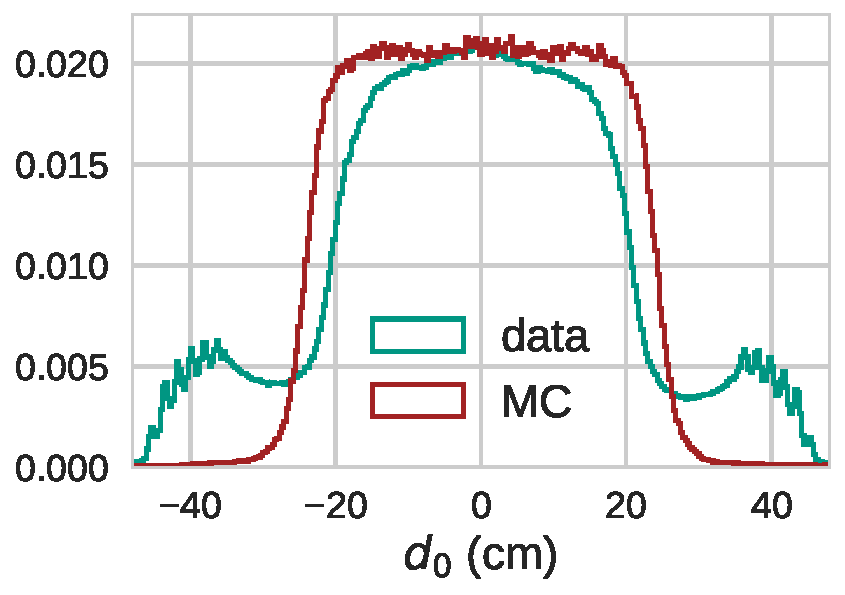
\includegraphics[width=0.3\textwidth]{figures/distributions/gcr_august_2017_d0_distribution_normed=True.pdf}\\
    \includegraphics[width=0.3\textwidth]{figures/distributions/gcr_august_2017_phi0_distribution_normed=True.pdf}
    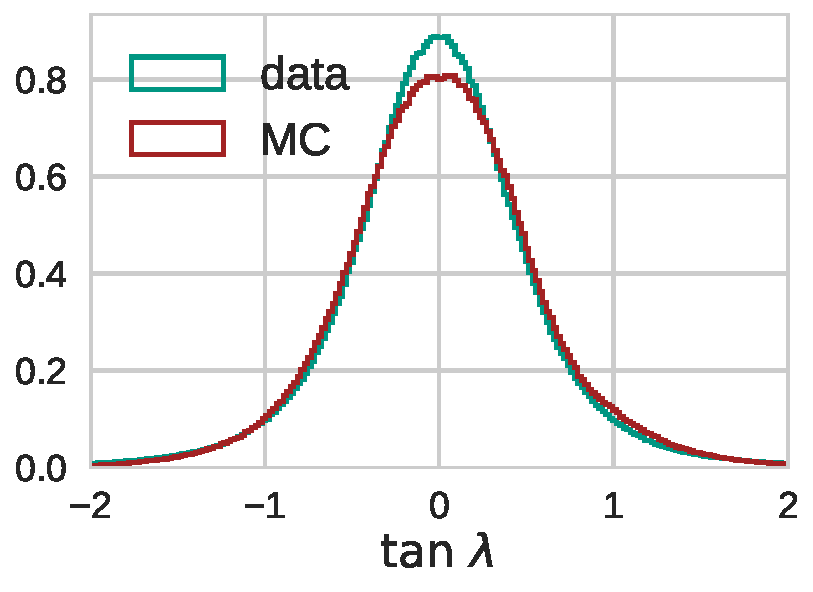
\includegraphics[width=0.3\textwidth]{figures/distributions/gcr_august_2017_tan_lambda_distribution_normed=True.pdf}
  \end{center}
\end{frame}

\begin{frame}
  \frametitle{Y(4S) event with background in CDC}
  \begin{center}
    % \includegraphics[width=0.8\textwidth]{figures/b2display_screenshots/y4s_nobackground_edited.png}
    \includegraphics[width=0.4\textwidth]{figures/cdc_2d_eventdisplay_background.png}
  \end{center}
\end{frame}

\begin{frame}
  \frametitle{CDC drift cell configuration}
  \begin{center}
    \includegraphics[width=0.4\textwidth]{figures/belle2_driftcell_configuration_fromnilsmaster.pdf}
  \end{center}
\end{frame}

\end{document}

%%% Local Variables:
%%% coding: utf-8
%%% mode: latex
%%% TeX-engine: default
%%% TeX-master: t
%%% End: